\documentclass[12pt,a4paper,leqno]{report}

\usepackage[T1]{fontenc}
\usepackage[english]{babel}
\usepackage{amsthm}
\usepackage{amsfonts}
\usepackage{amsmath}
\usepackage{amssymb}
\usepackage{tikz}
\usepackage{listings}
\usepackage{blindtext}
\usepackage{scrextend}
\usepackage{dirtytalk}

\newcommand{\R}{\mathbb{R}}
\newcommand{\C}{\mathbb{C}}
\newcommand{\Q}{\mathbb{Q}}
\newcommand{\N}{\mathbb{N}}
\newcommand{\No}{\mathbb{N}_0}
\newcommand{\Z}{\mathbb{Z}}
\newcommand{\diam}{\operatorname{diam}}

\theoremstyle{plain}
\newtheorem{equa}[equation]{Equation}
\newtheorem{lem}[equation]{Lemma}
\newtheorem{prop}[equation]{Proposition}
\newtheorem{cor}[equation]{Corollary}

\theoremstyle{definition}
\newtheorem{defi}[equation]{definition}
\newtheorem{conj}[equation]{Conjecture}
\newtheorem{example}[equation]{Example}
\theoremstyle{remark}
\newtheorem{note}[equation]{Note}

\pagestyle{plain}
\makeatletter
\renewcommand{\@seccntformat}[1]{}
\makeatother
\setcounter{page}{1}
\addtolength{\hoffset}{-1.15cm}
\addtolength{\textwidth}{2.3cm}
\addtolength{\voffset}{0.45cm}
\addtolength{\textheight}{-0.9cm}

\graphicspath{ {./figures/} }

\title{Data Analytics 5 - Default Risk Prediction}
\author{Tuomo Kareoja}
\date{}

\begin{document}

\maketitle

\begin{table}[h!]
  \begin{center}
    \begin{tabular}{l|c|r}
      \textbf{Version Number} & \textbf{Changes} & \textbf{Date} \\
      \hline
      0.8 & Finished plots and most of the text & 11.11.2019\\
      1.0 & Finished text and plots & 12.11.2019\\
    \end{tabular}
  \end{center}
\end{table}

\newpage

\section{Problem and Suggested Solution}

\begin{labeling}{something}
\item [\textbf{The Problem:}] The proportion of customers that we have set the credit limits to are defaulting
\item [\textbf{What We Can Do:}] The only leverage we have is the credit limit. Changing the credit limit downward
    for customers that have a high change of defaulting could create complaints and unlikely to work as the customer
    might have already taken enough dept to cause them to default and lowering the credit limit would not affect this.
    An another option would be to check that the credit limit given to customers is low enough from the get-go
\item [\textbf{Suggested Solution:}] Build a predictive model that can find the customers to whom we should be giving less
    credit and find how much should we lower the credit of these customers
\end{labeling}

\section{The Logic of the Solution}

Just finding the customers that are about to default is not enough,
because in the end we would like to prevent defaults from happening
and even if a customer has a high immediate risk of default we might
not have any leverage to change her behavior at this point. Where
we would have leverage is in the moment when we are setting
the customers credit limit before things escalated.

If we could find the customers where giving them a lower credit limit
would prevent their future default by preventing them from taking
a loan that too big for them to handle, we would have an option
to actually effect the outcome.

To find the customers where a lower credit limit would be appropriate
we need go trough the following steps:

\begin{enumerate}
    \item Clean and process data
    \item Build models that predict defaulting
    \item Vary the amount of credit given in the data and see how this affects
    the risk of defaulting
    \item Find the credit drops that lower the risk of defaulting most with
    the lowest drop in credit limit
    \item Rank credit limit drops and calculate how much would the percentage of
    defaulters change and how much credit would need to give up in percentage terms
    \item Calculate the percent of defaulters, non-defaulters and customers in
    general who would be affected
\end{enumerate}

Because the data that we use is so limited we would predict that
the results will not be spectacular, but this should be seen more
as a proof of concept.

\section{Clean and Process the data}

The data that we were given pertains to the immediate risk of defaulting,
but we can use this data to simulate a situation where we are
setting the customers their credit limits (probably years before the possible
default) by just considering the demographic information of the customer.

This is the information about the customer that we are left with after
dropping columns that do not fit our hypothetical use case:

\begin{itemize}
    \item sex
    \item age
    \item education
    \item marital status
    \item credit given
    \item default
\end{itemize}

14 customers had education or marital status coded as 0 that we assumed
meant missing. These observations were simply dropped, because their number was so
small to make no difference and this made rest of the analysis more simple.

\subsection{Building Models That Predict Defaulting}

We want to find the best model to predict defaulting with the data that we have.
For this purpose we tried three models: XGBoost, random forest and CatBoost.
Below are the of ROC-curves of the models, unfortunately the models are not
labeled in the legend, but blue is XGBoost, red is random forest and green
is CatBoost. We see that XGBoost are tied for the best place (AUC=0.64) and
that random forest performs significantly worse.

\bigskip
{
    \centering
    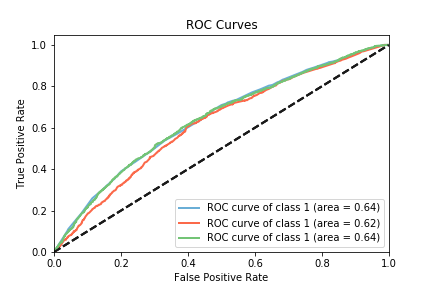
\includegraphics[width=\textwidth,height=\textheight,keepaspectratio]{roc_curves.png}
    \par
}
\bigskip

The next statistic to look is lift curve that tells us how much more likely defaulters
we would find by using the model and starting with the observations with the
highest predicted probability of defaulting versus using a random guess where we would
predict defaulting with the base rate of rate of defaulting.
As the percent of defaulters is around 20 \%, lift of 2 would mean that
the model would pick up 40 \% of the defaulters and that the random guess would
predict defaulting for random 20 \% of the customers.
The following plots are the lift curves for XGBoost and CatBoost models.
Here the lift rate is marked for both classes 0 and 1. We only care about
class 1 which means that the customer defaulted.
The following plots are the lift curves for XGBoost and CatBoost models. The
models perform very similarly except that CatBoost has high variance of
lift for the first couple of predictions.

\bigskip
{
    \centering
    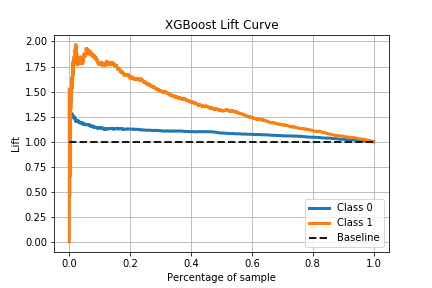
\includegraphics[scale=0.9]{xgboost_lift_curve.png}
    \par
}
\bigskip

\bigskip
{
    \centering
    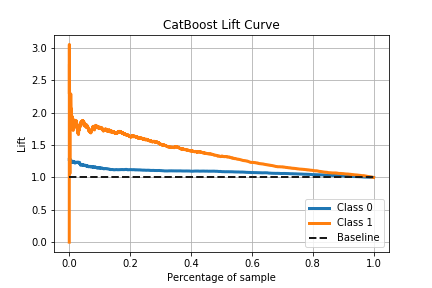
\includegraphics[scale=0.9]{catboost_lift_curve.png}
    \par
}
\bigskip

The last metric that we are interested in is how well the predicted probabilities
of the models match the real probabilities of defaulting. This means that for customers
where we predict a 60 \% chance of defaulting we want 60 \% of the customers to actually
default. We need these to be true as we are are handling these predictions as probabilities
to make further steps possible. We can see that all of the models predictions
line up quite nicely with actual probabilities. This was initially not case with
random forest model that had to tuned separately to have this feature.

\section{Finding the Customers and Credit Drops that Most Lower the Change of Defaulting}

Now that we have the models, the next step is to predict for each customer, how
big would the drop in the probability of defaulting be if we changed their
credit limit by certain percentage. To accomplish this we did the following

\begin{itemize}
    \item Train models with 80 \% of the data
    \item Use these trained models to predict the base chance of defaulting
    \item For each customer lower the actual credit limit by different percentages
    and see how this affects the predicted probability of defaulting
\end{itemize}

This is procedure was in principle quite simple, but the problem turned out to be that
the models didn't have the expected effect of credit limit for most customers.
To give an example of this, below are the all the features and their effects in
Shapley values for each customer for CatBoost. On the X-axis is the Shapley
value that is tells us was the effect of the variable value positive, and increasing
the probability of defaulting, or negative and decreasing the probability of defaulting.
We can se that for most customers (dots) low credit limit predicts higher probability
of defaulting. This obviously does not make sense, but if we consider the
variables that we are using there is logical reason for these results.

\bigskip
{
    \centering
    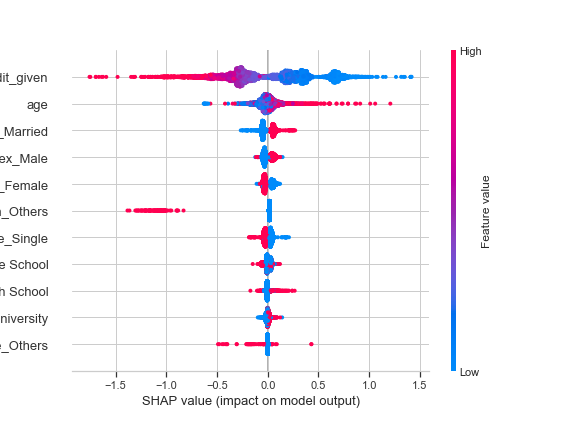
\includegraphics[width=\textwidth,height=\textheight,keepaspectratio]{catboost_shap_all_features.png}
    \par
}
\bigskip

When the credit limit is decided there are far more background variables taken into
account than we have access here. This means that we credit limit contains
lots of information about the credit worthiness of the customer that is not accounted
by the used demographic variables. So when the models is saying that higher
credit rating would lessen the the probability of defaulting, it actually means
that higher credit worthiness of the customer would lessen the probability of
defaulting.

Even though this is a big problem, there are still few customers where the models
would predict drops in defaulting probability with lower credit limit even with this
limited data. This means that even with this limited data we are able to capture
an effect that we would predict from background knowledge.


Even though the credit though the model would predict that a higher credit
limit would prevent defaults, this should not be the case for all customers
we would like to find the customer groups that even with the limited amount
of demographic data available have a credit limit that seems too high.

\section{Optimization of the Results}

Now that we calculated how the models predict dropping the credit limit affects the
defaulting probability for each customer we can move on to picking the optimal
customers and credit limit drops to get the maximum effect with smallest changes in
the overall credit issued. We did this with the following steps:

\begin{itemize}
    \item For each customer and credit limit drop, calculate the absolute loss
    in credit given divided by the percentage drop in defaulting probability. This
    gives us a cost for option in dollars per percentage drop
    \item for each customer find the most cost effective credit drop and calculate
    the cost of further drops in credit. This has to be done so that on top of
    considering drops for different customers we have possibilities in credit
    drop for each customer and these have to be made consecutively
    \item Put all these different drops in credit in order based on their costs, that
    is their cost in credit given per percentage drop in defaulting
\end{itemize}

Only the the results from CatBoost model were considered good. XGBoos model found
only around 20 customer (0.4 \% of customers in the test data), where lowering the
credit limit would also lower the risk of defaulting. Random forest predicted
drops in defaulting rate but, these were hovering around zero and seemed more
like random occurrences than real effect.

Below is a graph of how the number of steps of credit limiting affect
the percentage of defaults and credit given. Steps can be new customers
or further drops in the credit for customers where credit was already dropped.
We can see that for 1000 steps we would drop percentage of defaulters with
0.3 \% percentage points with a corresponding 1.5 \% drop in the total credit
given.

\bigskip
{
    \centering
    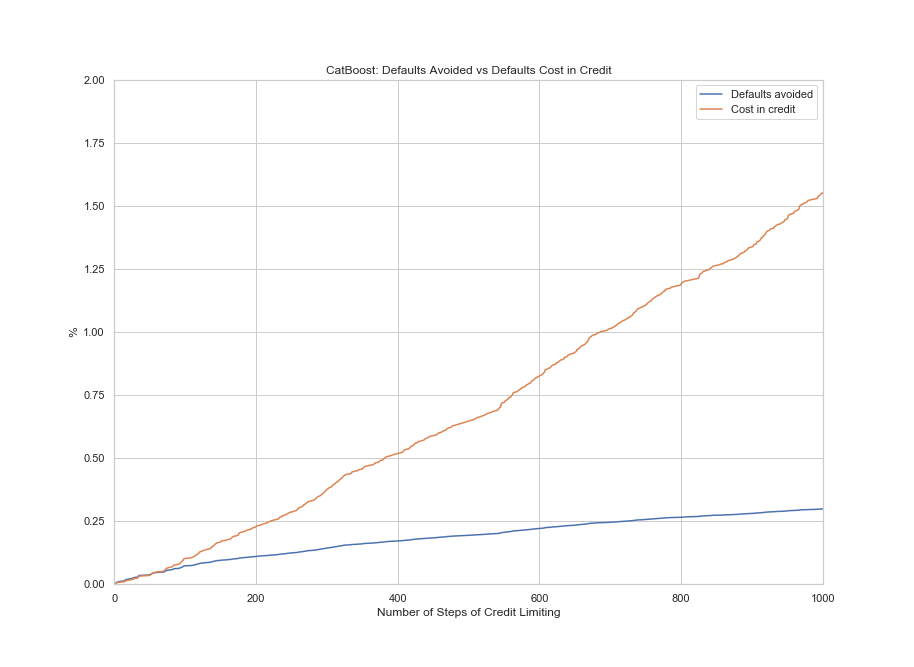
\includegraphics[width=\textwidth,height=\textheight,keepaspectratio]{catboost_defaults_vs_costs.png}
    \par
}
\bigskip

Here we can see how many percentage of customers would be effected in total and divided
to defaulters and non-defaulters. We see that for 1000 credit drops we would affect around
16 \% of the customers in test data (800 customers) with significantly higher
proportion of these drop hitting customers who actually defaulted.

\bigskip
{
    \centering
    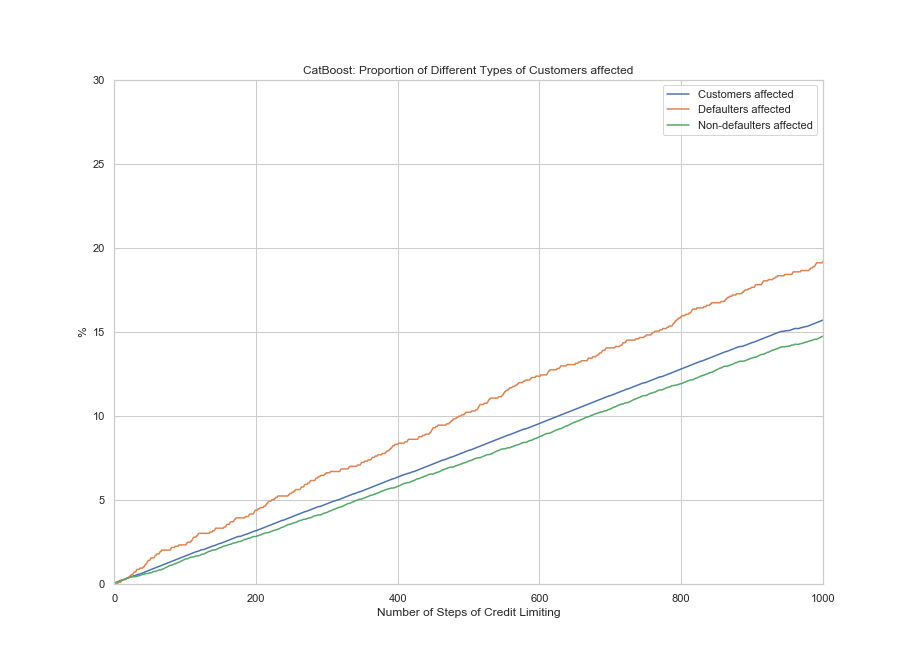
\includegraphics[width=\textwidth,height=\textheight,keepaspectratio]{catboost_types_of_customers_affected.png}
    \par
}
\bigskip

These results are not spectacular, but demonstrate the logic of the system.
With more data come better models and we should be able to prevent more
defaults with less drops and affect more of the would be defaulters than
non-defaulting customers.

\section{Next Steps}

\begin{labeling}{description}
\item [\textbf{1. Get Better Data}]
    The method for finding the customers where
    we should lower the credit limit
    works in concept, but for actual viability test we would need access to all
    the same data that are used by our employees to make the decisions about allowed
    credit limits.
\item [\textbf{2. Do a Proper Viability Test}] To do a proper of the viability of the
    concept we would need to have access to the same variables that are used when the
    credit limit is decided for building the models. Pay special attention in making
    sure that the causal link of credit limit and defaulting is tested properly
    (right direction, statistical tests, etc.)
\item [\textbf{3. Small Scale Test of Actual System}] The ultimate goal would be to
    create a system that could warn our employers when they are about to approve a credit
    limit that is too big and suggest them a suitably lower credit limit that is big
    enough to have a meaningful effect on the probability of default without denying
    the customer credit completely
\end{labeling}

\end{document}
